\documentclass[1p]{elsarticle_modified}
%\bibliographystyle{elsarticle-num}

%\usepackage[colorlinks]{hyperref}
%\usepackage{abbrmath_seonhwa} %\Abb, \Ascr, \Acal ,\Abf, \Afrak
\usepackage{amsfonts}
\usepackage{amssymb}
\usepackage{amsmath}
\usepackage{amsthm}
\usepackage{scalefnt}
\usepackage{amsbsy}
\usepackage{kotex}
\usepackage{caption}
\usepackage{subfig}
\usepackage{color}
\usepackage{graphicx}
\usepackage{xcolor} %% white, black, red, green, blue, cyan, magenta, yellow
\usepackage{float}
\usepackage{setspace}
\usepackage{hyperref}

\usepackage{tikz}
\usetikzlibrary{arrows}

\usepackage{multirow}
\usepackage{array} % fixed length table
\usepackage{hhline}

%%%%%%%%%%%%%%%%%%%%%
\makeatletter
\renewcommand*\env@matrix[1][\arraystretch]{%
	\edef\arraystretch{#1}%
	\hskip -\arraycolsep
	\let\@ifnextchar\new@ifnextchar
	\array{*\c@MaxMatrixCols c}}
\makeatother %https://tex.stackexchange.com/questions/14071/how-can-i-increase-the-line-spacing-in-a-matrix
%%%%%%%%%%%%%%%

\usepackage[normalem]{ulem}

\newcommand{\msout}[1]{\ifmmode\text{\sout{\ensuremath{#1}}}\else\sout{#1}\fi}
%SOURCE: \msout is \stkout macro in https://tex.stackexchange.com/questions/20609/strikeout-in-math-mode

\newcommand{\cancel}[1]{
	\ifmmode
	{\color{red}\msout{#1}}
	\else
	{\color{red}\sout{#1}}
	\fi
}

\newcommand{\add}[1]{
	{\color{blue}\uwave{#1}}
}

\newcommand{\replace}[2]{
	\ifmmode
	{\color{red}\msout{#1}}{\color{blue}\uwave{#2}}
	\else
	{\color{red}\sout{#1}}{\color{blue}\uwave{#2}}
	\fi
}

\newcommand{\Sol}{\mathcal{S}} %segment
\newcommand{\D}{D} %diagram
\newcommand{\A}{\mathcal{A}} %arc


%%%%%%%%%%%%%%%%%%%%%%%%%%%%%5 test

\def\sl{\operatorname{\textup{SL}}(2,\Cbb)}
\def\psl{\operatorname{\textup{PSL}}(2,\Cbb)}
\def\quan{\mkern 1mu \triangleright \mkern 1mu}

\theoremstyle{definition}
\newtheorem{thm}{Theorem}[section]
\newtheorem{prop}[thm]{Proposition}
\newtheorem{lem}[thm]{Lemma}
\newtheorem{ques}[thm]{Question}
\newtheorem{cor}[thm]{Corollary}
\newtheorem{defn}[thm]{Definition}
\newtheorem{exam}[thm]{Example}
\newtheorem{rmk}[thm]{Remark}
\newtheorem{alg}[thm]{Algorithm}

\newcommand{\I}{\sqrt{-1}}
\begin{document}

%\begin{frontmatter}
%
%\title{Boundary parabolic representations of knots up to 8 crossings}
%
%%% Group authors per affiliation:
%\author{Yunhi Cho} 
%\address{Department of Mathematics, University of Seoul, Seoul, Korea}
%\ead{yhcho@uos.ac.kr}
%
%
%\author{Seonhwa Kim} %\fnref{s_kim}}
%\address{Center for Geometry and Physics, Institute for Basic Science, Pohang, 37673, Korea}
%\ead{ryeona17@ibs.re.kr}
%
%\author{Hyuk Kim}
%\address{Department of Mathematical Sciences, Seoul National University, Seoul 08826, Korea}
%\ead{hyukkim@snu.ac.kr}
%
%\author{Seokbeom Yoon}
%\address{Department of Mathematical Sciences, Seoul National University, Seoul, 08826,  Korea}
%\ead{sbyoon15@snu.ac.kr}
%
%\begin{abstract}
%We find all boundary parabolic representation of knots up to 8 crossings.
%
%\end{abstract}
%\begin{keyword}
%    \MSC[2010] 57M25 
%\end{keyword}
%
%\end{frontmatter}

%\linenumbers
%\tableofcontents
%
\newcommand\colored[1]{\textcolor{white}{\rule[-0.35ex]{0.8em}{1.4ex}}\kern-0.8em\color{red} #1}%
%\newcommand\colored[1]{\textcolor{white}{ #1}\kern-2.17ex	\textcolor{white}{ #1}\kern-1.81ex	\textcolor{white}{ #1}\kern-2.15ex\color{red}#1	}

{\Large $\underline{12n_{0882}~(K12n_{0882})}$}

\setlength{\tabcolsep}{10pt}
\renewcommand{\arraystretch}{1.6}
\vspace{1cm}\begin{tabular}{m{100pt}>{\centering\arraybackslash}m{274pt}}
\multirow{5}{120pt}{
	\centering
	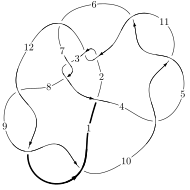
\includegraphics[width=112pt]{../../../GIT/diagram.site/Diagrams/png/2971_12n_0882.png}\\
\ \ \ A knot diagram\footnotemark}&
\allowdisplaybreaks
\textbf{Linearized knot diagam} \\
\cline{2-2}
 &
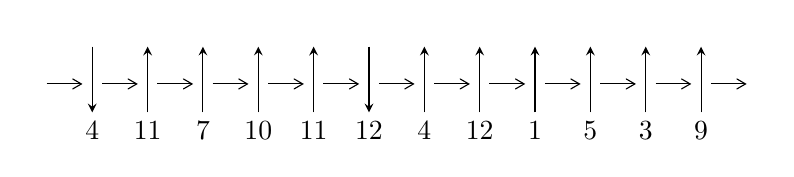
\begin{tikzpicture}[x=20pt, y=17pt]
	% nodes
	\node (C0) at (0, 0) {};
	\node (C1) at (1, 0) {};
	\node (C1U) at (1, +1) {};
	\node (C1D) at (1, -1) {4};

	\node (C2) at (2, 0) {};
	\node (C2U) at (2, +1) {};
	\node (C2D) at (2, -1) {11};

	\node (C3) at (3, 0) {};
	\node (C3U) at (3, +1) {};
	\node (C3D) at (3, -1) {7};

	\node (C4) at (4, 0) {};
	\node (C4U) at (4, +1) {};
	\node (C4D) at (4, -1) {10};

	\node (C5) at (5, 0) {};
	\node (C5U) at (5, +1) {};
	\node (C5D) at (5, -1) {11};

	\node (C6) at (6, 0) {};
	\node (C6U) at (6, +1) {};
	\node (C6D) at (6, -1) {12};

	\node (C7) at (7, 0) {};
	\node (C7U) at (7, +1) {};
	\node (C7D) at (7, -1) {4};

	\node (C8) at (8, 0) {};
	\node (C8U) at (8, +1) {};
	\node (C8D) at (8, -1) {12};

	\node (C9) at (9, 0) {};
	\node (C9U) at (9, +1) {};
	\node (C9D) at (9, -1) {1};

	\node (C10) at (10, 0) {};
	\node (C10U) at (10, +1) {};
	\node (C10D) at (10, -1) {5};

	\node (C11) at (11, 0) {};
	\node (C11U) at (11, +1) {};
	\node (C11D) at (11, -1) {3};

	\node (C12) at (12, 0) {};
	\node (C12U) at (12, +1) {};
	\node (C12D) at (12, -1) {9};
	\node (C13) at (13, 0) {};

	% arrows
	\draw[->,>={angle 60}]
	(C0) edge (C1) (C1) edge (C2) (C2) edge (C3) (C3) edge (C4) (C4) edge (C5) (C5) edge (C6) (C6) edge (C7) (C7) edge (C8) (C8) edge (C9) (C9) edge (C10) (C10) edge (C11) (C11) edge (C12) (C12) edge (C13) ;	\draw[->,>=stealth]
	(C1U) edge (C1D) (C2D) edge (C2U) (C3D) edge (C3U) (C4D) edge (C4U) (C5D) edge (C5U) (C6U) edge (C6D) (C7D) edge (C7U) (C8D) edge (C8U) (C9D) edge (C9U) (C10D) edge (C10U) (C11D) edge (C11U) (C12D) edge (C12U) ;
	\end{tikzpicture} \\
\hhline{~~} \\& 
\textbf{Solving Sequence} \\ \cline{2-2} 
 &
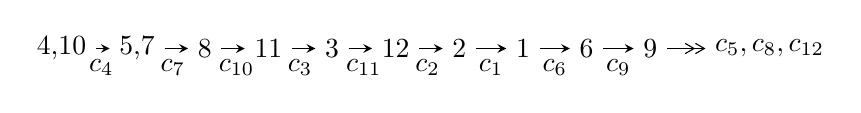
\begin{tikzpicture}[x=23pt, y=7pt]
	% node
	\node (A0) at (-1/8, 0) {4,10};
	\node (A1) at (17/16, 0) {5,7};
	\node (A2) at (17/8, 0) {8};
	\node (A3) at (25/8, 0) {11};
	\node (A4) at (33/8, 0) {3};
	\node (A5) at (41/8, 0) {12};
	\node (A6) at (49/8, 0) {2};
	\node (A7) at (57/8, 0) {1};
	\node (A8) at (65/8, 0) {6};
	\node (A9) at (73/8, 0) {9};
	\node (C1) at (1/2, -1) {$c_{4}$};
	\node (C2) at (13/8, -1) {$c_{7}$};
	\node (C3) at (21/8, -1) {$c_{10}$};
	\node (C4) at (29/8, -1) {$c_{3}$};
	\node (C5) at (37/8, -1) {$c_{11}$};
	\node (C6) at (45/8, -1) {$c_{2}$};
	\node (C7) at (53/8, -1) {$c_{1}$};
	\node (C8) at (61/8, -1) {$c_{6}$};
	\node (C9) at (69/8, -1) {$c_{9}$};
	\node (A10) at (11, 0) {$c_{5},c_{8},c_{12}$};

	% edge
	\draw[->,>=stealth]	
	(A0) edge (A1) (A1) edge (A2) (A2) edge (A3) (A3) edge (A4) (A4) edge (A5) (A5) edge (A6) (A6) edge (A7) (A7) edge (A8) (A8) edge (A9) ;
	\draw[->>,>={angle 60}]	
	(A9) edge (A10);
\end{tikzpicture} \\ 

\end{tabular} \\

\footnotetext{
The image of knot diagram is generated by the software ``\textbf{Draw programme}" developed by Andrew Bartholomew(\url{http://www.layer8.co.uk/maths/draw/index.htm\#Running-draw}), where we modified some parts for our purpose(\url{https://github.com/CATsTAILs/LinksPainter}).
}\phantom \\ \newline 
\centering \textbf{Ideals for irreducible components\footnotemark of $X_{\text{par}}$} 
 
\begin{align*}
I^u_{1}&=\langle 
4 u^{12}-8 u^{11}-26 u^{10}+41 u^9+59 u^8-69 u^7-42 u^6+9 u^5-10 u^4+56 u^3+u^2+13 b-5 u+10,\\
\phantom{I^u_{1}}&\phantom{= \langle  }-4 u^{12}+8 u^{11}+26 u^{10}-41 u^9-59 u^8+69 u^7+42 u^6-9 u^5+10 u^4-69 u^3- u^2+13 a+31 u-10,\\
\phantom{I^u_{1}}&\phantom{= \langle  }u^{13}+u^{12}-6 u^{11}-6 u^{10}+13 u^9+14 u^8-7 u^7-13 u^6-12 u^5+13 u^3+6 u^2+2 u+1\rangle \\
I^u_{2}&=\langle 
-5.18174\times10^{46} u^{47}-1.01683\times10^{47} u^{46}+\cdots+3.77343\times10^{47} b-4.53377\times10^{47},\\
\phantom{I^u_{2}}&\phantom{= \langle  }2.81502\times10^{47} u^{47}+3.21473\times10^{47} u^{46}+\cdots+1.25781\times10^{47} a+4.62967\times10^{48},\;u^{48}+u^{47}+\cdots+20 u+1\rangle \\
I^u_{3}&=\langle 
- u^2+b+1,\;- u^3+u^2+a+2 u-1,\;u^5-3 u^3+2 u+1\rangle \\
I^u_{4}&=\langle 
- u^2+b+1,\;-2 u^7- u^6+11 u^5+3 u^4-18 u^3+3 u^2+a+8 u-9,\\
\phantom{I^u_{4}}&\phantom{= \langle  }u^8-5 u^6+u^5+7 u^4-4 u^3-2 u^2+4 u-1\rangle \\
I^u_{5}&=\langle 
b+1,\;a,\;u-1\rangle \\
\\
\end{align*}
\raggedright * 5 irreducible components of $\dim_{\mathbb{C}}=0$, with total 75 representations.\\
\footnotetext{All coefficients of polynomials are rational numbers. But the coefficients are sometimes approximated in decimal forms when there is not enough margin.}
\newpage
\renewcommand{\arraystretch}{1}
\centering \section*{I. $I^u_{1}= \langle 4 u^{12}-8 u^{11}+\cdots+13 b+10,\;-4 u^{12}+8 u^{11}+\cdots+13 a-10,\;u^{13}+u^{12}+\cdots+2 u+1 \rangle$}
\flushleft \textbf{(i) Arc colorings}\\
\begin{tabular}{m{7pt} m{180pt} m{7pt} m{180pt} }
\flushright $a_{4}=$&$\begin{pmatrix}1\\0\end{pmatrix}$ \\
\flushright $a_{10}=$&$\begin{pmatrix}0\\u\end{pmatrix}$ \\
\flushright $a_{5}=$&$\begin{pmatrix}1\\- u^2\end{pmatrix}$ \\
\flushright $a_{7}=$&$\begin{pmatrix}0.307692 u^{12}-0.615385 u^{11}+\cdots-2.38462 u+0.769231\\-0.307692 u^{12}+0.615385 u^{11}+\cdots+0.384615 u-0.769231\end{pmatrix}$ \\
\flushright $a_{8}=$&$\begin{pmatrix}u^3-2 u\\-0.307692 u^{12}+0.615385 u^{11}+\cdots+0.384615 u-0.769231\end{pmatrix}$ \\
\flushright $a_{11}=$&$\begin{pmatrix}u\\- u^3+u\end{pmatrix}$ \\
\flushright $a_{3}=$&$\begin{pmatrix}0.538462 u^{12}-0.0769231 u^{11}+\cdots+3.07692 u+1.84615\\-1.07692 u^{12}+0.153846 u^{11}+\cdots-2.15385 u-0.692308\end{pmatrix}$ \\
\flushright $a_{12}=$&$\begin{pmatrix}u^2-1\\-0.692308 u^{12}+0.384615 u^{11}+\cdots+1.61538 u-0.230769\end{pmatrix}$ \\
\flushright $a_{2}=$&$\begin{pmatrix}1.46154 u^{12}+0.0769231 u^{11}+\cdots+2.92308 u+2.15385\\-1.46154 u^{12}-0.0769231 u^{11}+\cdots-2.92308 u-1.15385\end{pmatrix}$ \\
\flushright $a_{1}=$&$\begin{pmatrix}1\\-1.46154 u^{12}-0.0769231 u^{11}+\cdots-2.92308 u-1.15385\end{pmatrix}$ \\
\flushright $a_{6}=$&$\begin{pmatrix}- u^2+1\\u^4-2 u^2\end{pmatrix}$ \\
\flushright $a_{9}=$&$\begin{pmatrix}- u\\-1.38462 u^{12}+0.769231 u^{11}+\cdots-0.769231 u-1.46154\end{pmatrix}$\\&\end{tabular}
\flushleft \textbf{(ii) Obstruction class $= -1$}\\~\\
\flushleft \textbf{(iii) Cusp Shapes $= \frac{42}{13} u^{12}+\frac{20}{13} u^{11}-18 u^{10}-\frac{122}{13} u^9+\frac{483}{13} u^8+\frac{309}{13} u^7-\frac{285}{13} u^6-\frac{367}{13} u^5-\frac{300}{13} u^4+\frac{94}{13} u^3+\frac{394}{13} u^2+\frac{162}{13} u+\frac{157}{13}$}\\~\\
\newpage\renewcommand{\arraystretch}{1}
\flushleft \textbf{(iv) u-Polynomials at the component}\newline \\
\begin{tabular}{m{50pt}|m{274pt}}
Crossings & \hspace{64pt}u-Polynomials at each crossing \\
\hline $$\begin{aligned}c_{1}\end{aligned}$$&$\begin{aligned}
&u^{13}-12 u^{12}+\cdots+352 u-32
\end{aligned}$\\
\hline $$\begin{aligned}c_{2},c_{3},c_{7}\\c_{11}\end{aligned}$$&$\begin{aligned}
&u^{13}-3 u^{11}+9 u^9+u^8-12 u^7+u^6+16 u^5- u^4-11 u^3+3 u^2+4 u-1
\end{aligned}$\\
\hline $$\begin{aligned}c_{4},c_{5},c_{8}\\c_{9},c_{10},c_{12}\end{aligned}$$&$\begin{aligned}
&u^{13}- u^{12}+\cdots+2 u-1
\end{aligned}$\\
\hline $$\begin{aligned}c_{6}\end{aligned}$$&$\begin{aligned}
&u^{13}+11 u^{12}+\cdots-208 u-56
\end{aligned}$\\
\hline
\end{tabular}\\~\\
\newpage\renewcommand{\arraystretch}{1}
\flushleft \textbf{(v) Riley Polynomials at the component}\newline \\
\begin{tabular}{m{50pt}|m{274pt}}
Crossings & \hspace{64pt}Riley Polynomials at each crossing \\
\hline $$\begin{aligned}c_{1}\end{aligned}$$&$\begin{aligned}
&y^{13}+8 y^{12}+\cdots+42496 y-1024
\end{aligned}$\\
\hline $$\begin{aligned}c_{2},c_{3},c_{7}\\c_{11}\end{aligned}$$&$\begin{aligned}
&y^{13}-6 y^{12}+\cdots+22 y-1
\end{aligned}$\\
\hline $$\begin{aligned}c_{4},c_{5},c_{8}\\c_{9},c_{10},c_{12}\end{aligned}$$&$\begin{aligned}
&y^{13}-13 y^{12}+\cdots-8 y-1
\end{aligned}$\\
\hline $$\begin{aligned}c_{6}\end{aligned}$$&$\begin{aligned}
&y^{13}+y^{12}+\cdots+5408 y-3136
\end{aligned}$\\
\hline
\end{tabular}\\~\\
\newpage\flushleft \textbf{(vi) Complex Volumes and Cusp Shapes}
$$\begin{array}{c|c|c}  
\text{Solutions to }I^u_{1}& \I (\text{vol} + \sqrt{-1}CS) & \text{Cusp shape}\\
 \hline 
\begin{aligned}
u &= -0.171620 + 0.859681 I \\
a &= -0.34697 - 1.56070 I \\
b &= \phantom{-}1.065670 - 0.718049 I\end{aligned}
 & -2.17962 - 5.84511 I & \phantom{-}7.45794 + 6.04290 I \\ \hline\begin{aligned}
u &= -0.171620 - 0.859681 I \\
a &= -0.34697 + 1.56070 I \\
b &= \phantom{-}1.065670 + 0.718049 I\end{aligned}
 & -2.17962 + 5.84511 I & \phantom{-}7.45794 - 6.04290 I \\ \hline\begin{aligned}
u &= -1.309140 + 0.064534 I \\
a &= -0.581299 - 0.674191 I \\
b &= \phantom{-}0.972284 + 0.876654 I\end{aligned}
 & \phantom{-}8.82263 + 2.58229 I & \phantom{-}16.9820 - 3.0015 I \\ \hline\begin{aligned}
u &= -1.309140 - 0.064534 I \\
a &= -0.581299 + 0.674191 I \\
b &= \phantom{-}0.972284 - 0.876654 I\end{aligned}
 & \phantom{-}8.82263 - 2.58229 I & \phantom{-}16.9820 + 3.0015 I \\ \hline\begin{aligned}
u &= \phantom{-}1.356440 + 0.275517 I \\
a &= \phantom{-}0.256447 + 0.156488 I \\
b &= -0.782477 + 0.792358 I\end{aligned}
 & \phantom{-}5.13873 + 2.17385 I & \phantom{-}13.57691 - 0.52106 I \\ \hline\begin{aligned}
u &= \phantom{-}1.356440 - 0.275517 I \\
a &= \phantom{-}0.256447 - 0.156488 I \\
b &= -0.782477 - 0.792358 I\end{aligned}
 & \phantom{-}5.13873 - 2.17385 I & \phantom{-}13.57691 + 0.52106 I \\ \hline\begin{aligned}
u &= \phantom{-}1.356860 + 0.395151 I \\
a &= -1.72651 + 1.21374 I \\
b &= \phantom{-}0.875267 + 0.116755 I\end{aligned}
 & \phantom{-}9.39305 + 5.41911 I & \phantom{-}19.2364 - 4.1129 I \\ \hline\begin{aligned}
u &= \phantom{-}1.356860 - 0.395151 I \\
a &= -1.72651 - 1.21374 I \\
b &= \phantom{-}0.875267 - 0.116755 I\end{aligned}
 & \phantom{-}9.39305 - 5.41911 I & \phantom{-}19.2364 + 4.1129 I \\ \hline\begin{aligned}
u &= -0.537178\phantom{ +0.000000I} \\
a &= \phantom{-}1.16207\phantom{ +0.000000I} \\
b &= -0.242725\phantom{ +0.000000I}\end{aligned}
 & \phantom{-}0.805138\phantom{ +0.000000I} & \phantom{-}11.7720\phantom{ +0.000000I} \\ \hline\begin{aligned}
u &= -1.48836 + 0.39264 I \\
a &= \phantom{-}1.67676 + 0.98279 I \\
b &= -1.30871 + 0.78070 I\end{aligned}
 & \phantom{-}8.6054 - 15.1865 I & \phantom{-}15.2811 + 7.9689 I\\
 \hline 
 \end{array}$$\newpage$$\begin{array}{c|c|c}  
\text{Solutions to }I^u_{1}& \I (\text{vol} + \sqrt{-1}CS) & \text{Cusp shape}\\
 \hline 
\begin{aligned}
u &= -1.48836 - 0.39264 I \\
a &= \phantom{-}1.67676 - 0.98279 I \\
b &= -1.30871 - 0.78070 I\end{aligned}
 & \phantom{-}8.6054 + 15.1865 I & \phantom{-}15.2811 - 7.9689 I \\ \hline\begin{aligned}
u &= \phantom{-}0.024401 + 0.393610 I \\
a &= \phantom{-}0.640545 - 1.244220 I \\
b &= -0.700673 + 0.396722 I\end{aligned}
 & \phantom{-}1.07099 - 1.38837 I & \phantom{-}7.07977 + 4.85651 I \\ \hline\begin{aligned}
u &= \phantom{-}0.024401 - 0.393610 I \\
a &= \phantom{-}0.640545 + 1.244220 I \\
b &= -0.700673 - 0.396722 I\end{aligned}
 & \phantom{-}1.07099 + 1.38837 I & \phantom{-}7.07977 - 4.85651 I\\
 \hline 
 \end{array}$$\newpage\newpage\renewcommand{\arraystretch}{1}
\centering \section*{II. $I^u_{2}= \langle -5.18\times10^{46} u^{47}-1.02\times10^{47} u^{46}+\cdots+3.77\times10^{47} b-4.53\times10^{47},\;2.82\times10^{47} u^{47}+3.21\times10^{47} u^{46}+\cdots+1.26\times10^{47} a+4.63\times10^{48},\;u^{48}+u^{47}+\cdots+20 u+1 \rangle$}
\flushleft \textbf{(i) Arc colorings}\\
\begin{tabular}{m{7pt} m{180pt} m{7pt} m{180pt} }
\flushright $a_{4}=$&$\begin{pmatrix}1\\0\end{pmatrix}$ \\
\flushright $a_{10}=$&$\begin{pmatrix}0\\u\end{pmatrix}$ \\
\flushright $a_{5}=$&$\begin{pmatrix}1\\- u^2\end{pmatrix}$ \\
\flushright $a_{7}=$&$\begin{pmatrix}-2.23803 u^{47}-2.55582 u^{46}+\cdots-95.9559 u-36.8074\\0.137322 u^{47}+0.269470 u^{46}+\cdots+10.2860 u+1.20150\end{pmatrix}$ \\
\flushright $a_{8}=$&$\begin{pmatrix}-2.10071 u^{47}-2.28635 u^{46}+\cdots-85.6699 u-35.6059\\0.137322 u^{47}+0.269470 u^{46}+\cdots+10.2860 u+1.20150\end{pmatrix}$ \\
\flushright $a_{11}=$&$\begin{pmatrix}u\\- u^3+u\end{pmatrix}$ \\
\flushright $a_{3}=$&$\begin{pmatrix}-1.66504 u^{47}-1.59037 u^{46}+\cdots-127.758 u-32.3177\\0.0330654 u^{47}+0.122014 u^{46}+\cdots-10.8225 u+0.0377011\end{pmatrix}$ \\
\flushright $a_{12}=$&$\begin{pmatrix}-2.91125 u^{47}-2.61233 u^{46}+\cdots-182.706 u-53.5737\\0.168578 u^{47}+0.0577104 u^{46}+\cdots-0.407278 u+0.897363\end{pmatrix}$ \\
\flushright $a_{2}=$&$\begin{pmatrix}-1.68717 u^{47}-1.75245 u^{46}+\cdots-125.467 u-32.2876\\0.0461378 u^{47}+0.188914 u^{46}+\cdots-11.3519 u-0.0721935\end{pmatrix}$ \\
\flushright $a_{1}=$&$\begin{pmatrix}-1.64103 u^{47}-1.56354 u^{46}+\cdots-136.819 u-32.3598\\0.0461378 u^{47}+0.188914 u^{46}+\cdots-11.3519 u-0.0721935\end{pmatrix}$ \\
\flushright $a_{6}=$&$\begin{pmatrix}- u^2+1\\u^4-2 u^2\end{pmatrix}$ \\
\flushright $a_{9}=$&$\begin{pmatrix}2.76666 u^{47}+2.69855 u^{46}+\cdots+205.087 u+52.5080\\-0.111644 u^{47}+0.153944 u^{46}+\cdots+8.10592 u-0.451941\end{pmatrix}$\\&\end{tabular}
\flushleft \textbf{(ii) Obstruction class $= -1$}\\~\\
\flushleft \textbf{(iii) Cusp Shapes $= -2.00373 u^{47}-2.03203 u^{46}+\cdots-42.9306 u-8.93702$}\\~\\
\newpage\renewcommand{\arraystretch}{1}
\flushleft \textbf{(iv) u-Polynomials at the component}\newline \\
\begin{tabular}{m{50pt}|m{274pt}}
Crossings & \hspace{64pt}u-Polynomials at each crossing \\
\hline $$\begin{aligned}c_{1}\end{aligned}$$&$\begin{aligned}
&(u^{24}+2 u^{23}+\cdots-20 u-1)^{2}
\end{aligned}$\\
\hline $$\begin{aligned}c_{2},c_{3},c_{7}\\c_{11}\end{aligned}$$&$\begin{aligned}
&u^{48}- u^{47}+\cdots-197 u+73
\end{aligned}$\\
\hline $$\begin{aligned}c_{4},c_{5},c_{8}\\c_{9},c_{10},c_{12}\end{aligned}$$&$\begin{aligned}
&u^{48}- u^{47}+\cdots-20 u+1
\end{aligned}$\\
\hline $$\begin{aligned}c_{6}\end{aligned}$$&$\begin{aligned}
&(u^{24}-5 u^{23}+\cdots+15 u-1)^{2}
\end{aligned}$\\
\hline
\end{tabular}\\~\\
\newpage\renewcommand{\arraystretch}{1}
\flushleft \textbf{(v) Riley Polynomials at the component}\newline \\
\begin{tabular}{m{50pt}|m{274pt}}
Crossings & \hspace{64pt}Riley Polynomials at each crossing \\
\hline $$\begin{aligned}c_{1}\end{aligned}$$&$\begin{aligned}
&(y^{24}+4 y^{23}+\cdots-522 y+1)^{2}
\end{aligned}$\\
\hline $$\begin{aligned}c_{2},c_{3},c_{7}\\c_{11}\end{aligned}$$&$\begin{aligned}
&y^{48}-23 y^{47}+\cdots-76039 y+5329
\end{aligned}$\\
\hline $$\begin{aligned}c_{4},c_{5},c_{8}\\c_{9},c_{10},c_{12}\end{aligned}$$&$\begin{aligned}
&y^{48}-43 y^{47}+\cdots-216 y+1
\end{aligned}$\\
\hline $$\begin{aligned}c_{6}\end{aligned}$$&$\begin{aligned}
&(y^{24}-3 y^{23}+\cdots-135 y+1)^{2}
\end{aligned}$\\
\hline
\end{tabular}\\~\\
\newpage\flushleft \textbf{(vi) Complex Volumes and Cusp Shapes}
$$\begin{array}{c|c|c}  
\text{Solutions to }I^u_{2}& \I (\text{vol} + \sqrt{-1}CS) & \text{Cusp shape}\\
 \hline 
\begin{aligned}
u &= \phantom{-}0.379137 + 0.976493 I \\
a &= -0.471549 + 1.157640 I \\
b &= \phantom{-}1.29469 + 0.67005 I\end{aligned}
 & \phantom{-}2.67292 + 10.25690 I & \phantom{-}12.1975 - 7.6788 I \\ \hline\begin{aligned}
u &= \phantom{-}0.379137 - 0.976493 I \\
a &= -0.471549 - 1.157640 I \\
b &= \phantom{-}1.29469 - 0.67005 I\end{aligned}
 & \phantom{-}2.67292 - 10.25690 I & \phantom{-}12.1975 + 7.6788 I \\ \hline\begin{aligned}
u &= -0.021423 + 0.948358 I \\
a &= \phantom{-}0.401732 + 0.737665 I \\
b &= -0.856499 + 0.135005 I\end{aligned}
 & \phantom{-}4.94291 - 0.58720 I & \phantom{-}16.0412 - 0.8168 I \\ \hline\begin{aligned}
u &= -0.021423 - 0.948358 I \\
a &= \phantom{-}0.401732 - 0.737665 I \\
b &= -0.856499 - 0.135005 I\end{aligned}
 & \phantom{-}4.94291 + 0.58720 I & \phantom{-}16.0412 + 0.8168 I \\ \hline\begin{aligned}
u &= -1.023260 + 0.490646 I \\
a &= \phantom{-}0.476231 + 0.027830 I \\
b &= -1.044720 - 0.584882 I\end{aligned}
 & \phantom{-}0.464120 + 1.081590 I & \phantom{-}8.00000 - 2.00672 I \\ \hline\begin{aligned}
u &= -1.023260 - 0.490646 I \\
a &= \phantom{-}0.476231 - 0.027830 I \\
b &= -1.044720 + 0.584882 I\end{aligned}
 & \phantom{-}0.464120 - 1.081590 I & \phantom{-}8.00000 + 2.00672 I \\ \hline\begin{aligned}
u &= -0.379291 + 0.739173 I \\
a &= \phantom{-}0.316811 + 0.748267 I \\
b &= \phantom{-}0.248462 + 1.064600 I\end{aligned}
 & -0.51929 - 4.00862 I & \phantom{-}8.65058 + 5.80685 I \\ \hline\begin{aligned}
u &= -0.379291 - 0.739173 I \\
a &= \phantom{-}0.316811 - 0.748267 I \\
b &= \phantom{-}0.248462 - 1.064600 I\end{aligned}
 & -0.51929 + 4.00862 I & \phantom{-}8.65058 - 5.80685 I \\ \hline\begin{aligned}
u &= \phantom{-}1.135680 + 0.336882 I \\
a &= \phantom{-}0.864140 - 0.699527 I \\
b &= -0.713544 - 0.730081 I\end{aligned}
 & -0.51929 + 4.00862 I & \phantom{-}8.00000 - 5.80685 I \\ \hline\begin{aligned}
u &= \phantom{-}1.135680 - 0.336882 I \\
a &= \phantom{-}0.864140 + 0.699527 I \\
b &= -0.713544 + 0.730081 I\end{aligned}
 & -0.51929 - 4.00862 I & \phantom{-}8.00000 + 5.80685 I\\
 \hline 
 \end{array}$$\newpage$$\begin{array}{c|c|c}  
\text{Solutions to }I^u_{2}& \I (\text{vol} + \sqrt{-1}CS) & \text{Cusp shape}\\
 \hline 
\begin{aligned}
u &= -0.750478 + 0.292577 I \\
a &= \phantom{-}1.176600 + 0.468222 I \\
b &= -0.319389 + 0.477318 I\end{aligned}
 & \phantom{-}0.664158\phantom{ +0.000000I} & \phantom{-}9.39053 + 0. I\phantom{ +0.000000I} \\ \hline\begin{aligned}
u &= -0.750478 - 0.292577 I \\
a &= \phantom{-}1.176600 - 0.468222 I \\
b &= -0.319389 - 0.477318 I\end{aligned}
 & \phantom{-}0.664158\phantom{ +0.000000I} & \phantom{-}9.39053 + 0. I\phantom{ +0.000000I} \\ \hline\begin{aligned}
u &= \phantom{-}1.163220 + 0.303346 I \\
a &= -0.223618 - 0.467491 I \\
b &= -1.004700 + 0.471049 I\end{aligned}
 & \phantom{-}4.64466\phantom{ +0.000000I} & \phantom{-}15.0647 + 0. I\phantom{ +0.000000I} \\ \hline\begin{aligned}
u &= \phantom{-}1.163220 - 0.303346 I \\
a &= -0.223618 + 0.467491 I \\
b &= -1.004700 - 0.471049 I\end{aligned}
 & \phantom{-}4.64466\phantom{ +0.000000I} & \phantom{-}15.0647 + 0. I\phantom{ +0.000000I} \\ \hline\begin{aligned}
u &= \phantom{-}0.141459 + 0.765036 I \\
a &= \phantom{-}0.561104 - 0.769052 I \\
b &= \phantom{-}0.623240 - 0.846147 I\end{aligned}
 & -3.53422\phantom{ +0.000000I} & \phantom{-}4.26168 + 0. I\phantom{ +0.000000I} \\ \hline\begin{aligned}
u &= \phantom{-}0.141459 - 0.765036 I \\
a &= \phantom{-}0.561104 + 0.769052 I \\
b &= \phantom{-}0.623240 + 0.846147 I\end{aligned}
 & -3.53422\phantom{ +0.000000I} & \phantom{-}4.26168 + 0. I\phantom{ +0.000000I} \\ \hline\begin{aligned}
u &= \phantom{-}0.068175 + 0.762824 I \\
a &= \phantom{-}0.696604 + 1.029800 I \\
b &= \phantom{-}0.970507 + 0.650047 I\end{aligned}
 & \phantom{-}1.27885 + 3.92180 I & \phantom{-}9.29302 - 3.73808 I \\ \hline\begin{aligned}
u &= \phantom{-}0.068175 - 0.762824 I \\
a &= \phantom{-}0.696604 - 1.029800 I \\
b &= \phantom{-}0.970507 - 0.650047 I\end{aligned}
 & \phantom{-}1.27885 - 3.92180 I & \phantom{-}9.29302 + 3.73808 I \\ \hline\begin{aligned}
u &= \phantom{-}1.235930 + 0.167013 I \\
a &= -0.657445 - 0.412560 I \\
b &= \phantom{-}0.705420 + 0.391760 I\end{aligned}
 & \phantom{-}4.65694 + 3.47868 I & \phantom{-0.000000 } 0 \\ \hline\begin{aligned}
u &= \phantom{-}1.235930 - 0.167013 I \\
a &= -0.657445 + 0.412560 I \\
b &= \phantom{-}0.705420 - 0.391760 I\end{aligned}
 & \phantom{-}4.65694 - 3.47868 I & \phantom{-0.000000 } 0\\
 \hline 
 \end{array}$$\newpage$$\begin{array}{c|c|c}  
\text{Solutions to }I^u_{2}& \I (\text{vol} + \sqrt{-1}CS) & \text{Cusp shape}\\
 \hline 
\begin{aligned}
u &= \phantom{-}0.916403 + 0.885493 I \\
a &= \phantom{-}0.391708 - 0.248635 I \\
b &= -1.329710 + 0.460814 I\end{aligned}
 & \phantom{-}4.14619 - 4.10761 I & \phantom{-0.000000 } 0 \\ \hline\begin{aligned}
u &= \phantom{-}0.916403 - 0.885493 I \\
a &= \phantom{-}0.391708 + 0.248635 I \\
b &= -1.329710 - 0.460814 I\end{aligned}
 & \phantom{-}4.14619 + 4.10761 I & \phantom{-0.000000 } 0 \\ \hline\begin{aligned}
u &= -1.265470 + 0.153865 I \\
a &= -2.80490 - 0.73050 I \\
b &= \phantom{-}0.791562 + 0.363762 I\end{aligned}
 & \phantom{-}4.94291 - 0.58720 I & \phantom{-0.000000 } 0 \\ \hline\begin{aligned}
u &= -1.265470 - 0.153865 I \\
a &= -2.80490 + 0.73050 I \\
b &= \phantom{-}0.791562 - 0.363762 I\end{aligned}
 & \phantom{-}4.94291 + 0.58720 I & \phantom{-0.000000 } 0 \\ \hline\begin{aligned}
u &= -1.263720 + 0.231617 I \\
a &= \phantom{-}2.48042 + 2.19572 I \\
b &= -0.811085 + 0.535687 I\end{aligned}
 & \phantom{-}4.14619 - 4.10761 I & \phantom{-0.000000 } 0 \\ \hline\begin{aligned}
u &= -1.263720 - 0.231617 I \\
a &= \phantom{-}2.48042 - 2.19572 I \\
b &= -0.811085 - 0.535687 I\end{aligned}
 & \phantom{-}4.14619 + 4.10761 I & \phantom{-0.000000 } 0 \\ \hline\begin{aligned}
u &= -1.28856\phantom{ +0.000000I} \\
a &= -0.869778\phantom{ +0.000000I} \\
b &= -0.755603\phantom{ +0.000000I}\end{aligned}
 & \phantom{-}14.0810\phantom{ +0.000000I} & \phantom{-}25.5770\phantom{ +0.000000I} \\ \hline\begin{aligned}
u &= \phantom{-}1.32785\phantom{ +0.000000I} \\
a &= \phantom{-}4.15788\phantom{ +0.000000I} \\
b &= -0.885530\phantom{ +0.000000I}\end{aligned}
 & \phantom{-}14.6478\phantom{ +0.000000I} & \phantom{-0.000000 } 0 \\ \hline\begin{aligned}
u &= \phantom{-}1.330000 + 0.048649 I \\
a &= -2.39749 + 0.12309 I \\
b &= \phantom{-}1.065850 + 0.841425 I\end{aligned}
 & \phantom{-}9.08685 + 4.24572 I & \phantom{-0.000000 } 0 \\ \hline\begin{aligned}
u &= \phantom{-}1.330000 - 0.048649 I \\
a &= -2.39749 - 0.12309 I \\
b &= \phantom{-}1.065850 - 0.841425 I\end{aligned}
 & \phantom{-}9.08685 - 4.24572 I & \phantom{-0.000000 } 0\\
 \hline 
 \end{array}$$\newpage$$\begin{array}{c|c|c}  
\text{Solutions to }I^u_{2}& \I (\text{vol} + \sqrt{-1}CS) & \text{Cusp shape}\\
 \hline 
\begin{aligned}
u &= -1.309300 + 0.318007 I \\
a &= \phantom{-}0.889440 + 0.821935 I \\
b &= -0.928244 + 0.711653 I\end{aligned}
 & \phantom{-}5.58448 - 7.81589 I & \phantom{-0.000000 } 0 \\ \hline\begin{aligned}
u &= -1.309300 - 0.318007 I \\
a &= \phantom{-}0.889440 - 0.821935 I \\
b &= -0.928244 - 0.711653 I\end{aligned}
 & \phantom{-}5.58448 + 7.81589 I & \phantom{-0.000000 } 0 \\ \hline\begin{aligned}
u &= -1.316980 + 0.405826 I \\
a &= -0.548637 + 0.081279 I \\
b &= \phantom{-}0.803853 + 0.148006 I\end{aligned}
 & \phantom{-}9.08685 - 4.24572 I & \phantom{-0.000000 } 0 \\ \hline\begin{aligned}
u &= -1.316980 - 0.405826 I \\
a &= -0.548637 - 0.081279 I \\
b &= \phantom{-}0.803853 - 0.148006 I\end{aligned}
 & \phantom{-}9.08685 + 4.24572 I & \phantom{-0.000000 } 0 \\ \hline\begin{aligned}
u &= -0.087131 + 0.611347 I \\
a &= \phantom{-}0.35264 + 2.45893 I \\
b &= \phantom{-}0.721176 + 0.611639 I\end{aligned}
 & \phantom{-}0.464120 + 1.081590 I & \phantom{-}8.16075 - 2.00672 I \\ \hline\begin{aligned}
u &= -0.087131 - 0.611347 I \\
a &= \phantom{-}0.35264 - 2.45893 I \\
b &= \phantom{-}0.721176 - 0.611639 I\end{aligned}
 & \phantom{-}0.464120 - 1.081590 I & \phantom{-}8.16075 + 2.00672 I \\ \hline\begin{aligned}
u &= -1.373810 + 0.321857 I \\
a &= -0.344264 + 0.528075 I \\
b &= -0.621802 - 0.993232 I\end{aligned}
 & \phantom{-}1.27885 - 3.92180 I & \phantom{-0.000000 } 0 \\ \hline\begin{aligned}
u &= -1.373810 - 0.321857 I \\
a &= -0.344264 - 0.528075 I \\
b &= -0.621802 + 0.993232 I\end{aligned}
 & \phantom{-}1.27885 + 3.92180 I & \phantom{-0.000000 } 0 \\ \hline\begin{aligned}
u &= \phantom{-}1.36990 + 0.36882 I \\
a &= \phantom{-}1.75795 - 1.37725 I \\
b &= -1.073560 - 0.763448 I\end{aligned}
 & \phantom{-}2.67292 + 10.25690 I & \phantom{-0.000000 } 0 \\ \hline\begin{aligned}
u &= \phantom{-}1.36990 - 0.36882 I \\
a &= \phantom{-}1.75795 + 1.37725 I \\
b &= -1.073560 + 0.763448 I\end{aligned}
 & \phantom{-}2.67292 - 10.25690 I & \phantom{-0.000000 } 0\\
 \hline 
 \end{array}$$\newpage$$\begin{array}{c|c|c}  
\text{Solutions to }I^u_{2}& \I (\text{vol} + \sqrt{-1}CS) & \text{Cusp shape}\\
 \hline 
\begin{aligned}
u &= \phantom{-}1.49633 + 0.29266 I \\
a &= -0.376487 - 0.561865 I \\
b &= -0.34302 + 1.38502 I\end{aligned}
 & \phantom{-}5.58448 + 7.81589 I & \phantom{-0.000000 } 0 \\ \hline\begin{aligned}
u &= \phantom{-}1.49633 - 0.29266 I \\
a &= -0.376487 + 0.561865 I \\
b &= -0.34302 - 1.38502 I\end{aligned}
 & \phantom{-}5.58448 - 7.81589 I & \phantom{-0.000000 } 0 \\ \hline\begin{aligned}
u &= \phantom{-}1.65947\phantom{ +0.000000I} \\
a &= -1.72670\phantom{ +0.000000I} \\
b &= \phantom{-}1.72233\phantom{ +0.000000I}\end{aligned}
 & \phantom{-}10.1445\phantom{ +0.000000I} & \phantom{-0.000000 } 0 \\ \hline\begin{aligned}
u &= -1.66105\phantom{ +0.000000I} \\
a &= -1.80640\phantom{ +0.000000I} \\
b &= \phantom{-}2.14588\phantom{ +0.000000I}\end{aligned}
 & \phantom{-}14.0810\phantom{ +0.000000I} & \phantom{-0.000000 } 0 \\ \hline\begin{aligned}
u &= -1.81988\phantom{ +0.000000I} \\
a &= -1.44716\phantom{ +0.000000I} \\
b &= \phantom{-}1.67660\phantom{ +0.000000I}\end{aligned}
 & \phantom{-}14.6478\phantom{ +0.000000I} & \phantom{-0.000000 } 0 \\ \hline\begin{aligned}
u &= -0.024167 + 0.177554 I \\
a &= -0.54655 + 4.54825 I \\
b &= -1.041510 + 0.853951 I\end{aligned}
 & \phantom{-}4.65694 - 3.47868 I & \phantom{-}16.3031 + 8.4838 I \\ \hline\begin{aligned}
u &= -0.024167 - 0.177554 I \\
a &= -0.54655 - 4.54825 I \\
b &= -1.041510 - 0.853951 I\end{aligned}
 & \phantom{-}4.65694 + 3.47868 I & \phantom{-}16.3031 - 8.4838 I \\ \hline\begin{aligned}
u &= -0.0602179\phantom{ +0.000000I} \\
a &= -35.2967\phantom{ +0.000000I} \\
b &= \phantom{-}0.822371\phantom{ +0.000000I}\end{aligned}
 & \phantom{-}10.1445\phantom{ +0.000000I} & -9.41450\phantom{ +0.000000I}\\
 \hline 
 \end{array}$$\newpage\newpage\renewcommand{\arraystretch}{1}
\centering \section*{III. $I^u_{3}= \langle - u^2+b+1,\;- u^3+u^2+a+2 u-1,\;u^5-3 u^3+2 u+1 \rangle$}
\flushleft \textbf{(i) Arc colorings}\\
\begin{tabular}{m{7pt} m{180pt} m{7pt} m{180pt} }
\flushright $a_{4}=$&$\begin{pmatrix}1\\0\end{pmatrix}$ \\
\flushright $a_{10}=$&$\begin{pmatrix}0\\u\end{pmatrix}$ \\
\flushright $a_{5}=$&$\begin{pmatrix}1\\- u^2\end{pmatrix}$ \\
\flushright $a_{7}=$&$\begin{pmatrix}u^3- u^2-2 u+1\\u^2-1\end{pmatrix}$ \\
\flushright $a_{8}=$&$\begin{pmatrix}u^3-2 u\\u^2-1\end{pmatrix}$ \\
\flushright $a_{11}=$&$\begin{pmatrix}u\\- u^3+u\end{pmatrix}$ \\
\flushright $a_{3}=$&$\begin{pmatrix}- u^4+2 u^2-1\\u^4-2 u^2+1\end{pmatrix}$ \\
\flushright $a_{12}=$&$\begin{pmatrix}u^2-1\\- u^3- u^2+2 u+1\end{pmatrix}$ \\
\flushright $a_{2}=$&$\begin{pmatrix}- u^4- u^3+2 u^2+u-1\\u^4+u^3-2 u^2- u\end{pmatrix}$ \\
\flushright $a_{1}=$&$\begin{pmatrix}-1\\u^4+u^3-2 u^2- u\end{pmatrix}$ \\
\flushright $a_{6}=$&$\begin{pmatrix}- u^2+1\\u^4-2 u^2\end{pmatrix}$ \\
\flushright $a_{9}=$&$\begin{pmatrix}- u\\u^4+u^3- u^2- u-1\end{pmatrix}$\\&\end{tabular}
\flushleft \textbf{(ii) Obstruction class $= 1$}\\~\\
\flushleft \textbf{(iii) Cusp Shapes $= -2 u^4-3 u^3+3 u^2+2 u+17$}\\~\\
\newpage\renewcommand{\arraystretch}{1}
\flushleft \textbf{(iv) u-Polynomials at the component}\newline \\
\begin{tabular}{m{50pt}|m{274pt}}
Crossings & \hspace{64pt}u-Polynomials at each crossing \\
\hline $$\begin{aligned}c_{1}\end{aligned}$$&$\begin{aligned}
&u^5-2 u^4+5 u^3-4 u^2-1
\end{aligned}$\\
\hline $$\begin{aligned}c_{2},c_{7}\end{aligned}$$&$\begin{aligned}
&u^5+u^4- u^3- u^2+1
\end{aligned}$\\
\hline $$\begin{aligned}c_{3},c_{11}\end{aligned}$$&$\begin{aligned}
&u^5- u^4- u^3+u^2-1
\end{aligned}$\\
\hline $$\begin{aligned}c_{4},c_{5},c_{8}\\c_{9}\end{aligned}$$&$\begin{aligned}
&u^5-3 u^3+2 u+1
\end{aligned}$\\
\hline $$\begin{aligned}c_{6}\end{aligned}$$&$\begin{aligned}
&u^5+2 u^4+3 u^3+3 u^2+3 u+1
\end{aligned}$\\
\hline $$\begin{aligned}c_{10},c_{12}\end{aligned}$$&$\begin{aligned}
&u^5-3 u^3+2 u-1
\end{aligned}$\\
\hline
\end{tabular}\\~\\
\newpage\renewcommand{\arraystretch}{1}
\flushleft \textbf{(v) Riley Polynomials at the component}\newline \\
\begin{tabular}{m{50pt}|m{274pt}}
Crossings & \hspace{64pt}Riley Polynomials at each crossing \\
\hline $$\begin{aligned}c_{1}\end{aligned}$$&$\begin{aligned}
&y^5+6 y^4+9 y^3-20 y^2-8 y-1
\end{aligned}$\\
\hline $$\begin{aligned}c_{2},c_{3},c_{7}\\c_{11}\end{aligned}$$&$\begin{aligned}
&y^5-3 y^4+3 y^3-3 y^2+2 y-1
\end{aligned}$\\
\hline $$\begin{aligned}c_{4},c_{5},c_{8}\\c_{9},c_{10},c_{12}\end{aligned}$$&$\begin{aligned}
&y^5-6 y^4+13 y^3-12 y^2+4 y-1
\end{aligned}$\\
\hline $$\begin{aligned}c_{6}\end{aligned}$$&$\begin{aligned}
&y^5+2 y^4+3 y^3+5 y^2+3 y-1
\end{aligned}$\\
\hline
\end{tabular}\\~\\
\newpage\flushleft \textbf{(vi) Complex Volumes and Cusp Shapes}
$$\begin{array}{c|c|c}  
\text{Solutions to }I^u_{3}& \I (\text{vol} + \sqrt{-1}CS) & \text{Cusp shape}\\
 \hline 
\begin{aligned}
u &= \phantom{-}1.297630 + 0.272489 I \\
a &= -1.308900 + 0.104091 I \\
b &= \phantom{-}0.609585 + 0.707177 I\end{aligned}
 & \phantom{-}7.56155 + 5.69445 I & \phantom{-}14.5549 - 5.9553 I \\ \hline\begin{aligned}
u &= \phantom{-}1.297630 - 0.272489 I \\
a &= -1.308900 - 0.104091 I \\
b &= \phantom{-}0.609585 - 0.707177 I\end{aligned}
 & \phantom{-}7.56155 - 5.69445 I & \phantom{-}14.5549 + 5.9553 I \\ \hline\begin{aligned}
u &= -0.516079 + 0.312340 I \\
a &= \phantom{-}1.87697 - 0.08320 I \\
b &= -0.831219 - 0.322384 I\end{aligned}
 & \phantom{-}2.00050 + 0.85728 I & \phantom{-}16.5843 - 0.7821 I \\ \hline\begin{aligned}
u &= -0.516079 - 0.312340 I \\
a &= \phantom{-}1.87697 + 0.08320 I \\
b &= -0.831219 + 0.322384 I\end{aligned}
 & \phantom{-}2.00050 - 0.85728 I & \phantom{-}16.5843 + 0.7821 I \\ \hline\begin{aligned}
u &= -1.56310\phantom{ +0.000000I} \\
a &= -2.13614\phantom{ +0.000000I} \\
b &= \phantom{-}1.44327\phantom{ +0.000000I}\end{aligned}
 & \phantom{-}17.0644\phantom{ +0.000000I} & \phantom{-}20.7220\phantom{ +0.000000I}\\
 \hline 
 \end{array}$$\newpage\newpage\renewcommand{\arraystretch}{1}
\centering \section*{IV. $I^u_{4}= \langle - u^2+b+1,\;-2 u^7- u^6+\cdots+a-9,\;u^8-5 u^6+u^5+7 u^4-4 u^3-2 u^2+4 u-1 \rangle$}
\flushleft \textbf{(i) Arc colorings}\\
\begin{tabular}{m{7pt} m{180pt} m{7pt} m{180pt} }
\flushright $a_{4}=$&$\begin{pmatrix}1\\0\end{pmatrix}$ \\
\flushright $a_{10}=$&$\begin{pmatrix}0\\u\end{pmatrix}$ \\
\flushright $a_{5}=$&$\begin{pmatrix}1\\- u^2\end{pmatrix}$ \\
\flushright $a_{7}=$&$\begin{pmatrix}2 u^7+u^6-11 u^5-3 u^4+18 u^3-3 u^2-8 u+9\\u^2-1\end{pmatrix}$ \\
\flushright $a_{8}=$&$\begin{pmatrix}2 u^7+u^6-11 u^5-3 u^4+18 u^3-2 u^2-8 u+8\\u^2-1\end{pmatrix}$ \\
\flushright $a_{11}=$&$\begin{pmatrix}u\\- u^3+u\end{pmatrix}$ \\
\flushright $a_{3}=$&$\begin{pmatrix}-3 u^7- u^6+14 u^5+u^4-18 u^3+6 u^2+6 u-7\\u^4-2 u^2+1\end{pmatrix}$ \\
\flushright $a_{12}=$&$\begin{pmatrix}4 u^7+2 u^6-19 u^5-5 u^4+26 u^3-5 u^2-11 u+12\\u^5-4 u^3+u^2+3 u-2\end{pmatrix}$ \\
\flushright $a_{2}=$&$\begin{pmatrix}-3 u^7+14 u^5-2 u^4-17 u^3+7 u^2+4 u-7\\- u^6+4 u^4- u^3-3 u^2+2 u\end{pmatrix}$ \\
\flushright $a_{1}=$&$\begin{pmatrix}-3 u^7- u^6+14 u^5+2 u^4-18 u^3+4 u^2+6 u-7\\- u^6+4 u^4- u^3-3 u^2+2 u\end{pmatrix}$ \\
\flushright $a_{6}=$&$\begin{pmatrix}- u^2+1\\u^4-2 u^2\end{pmatrix}$ \\
\flushright $a_{9}=$&$\begin{pmatrix}-3 u^7+15 u^5-2 u^4-21 u^3+9 u^2+7 u-11\\u^7+u^6-4 u^5-3 u^4+4 u^3+u^2- u+1\end{pmatrix}$\\&\end{tabular}
\flushleft \textbf{(ii) Obstruction class $= 1$}\\~\\
\flushleft \textbf{(iii) Cusp Shapes $= 10 u^7+5 u^6-45 u^5-10 u^4+60 u^3-15 u^2-25 u+42$}\\~\\
\newpage\renewcommand{\arraystretch}{1}
\flushleft \textbf{(iv) u-Polynomials at the component}\newline \\
\begin{tabular}{m{50pt}|m{274pt}}
Crossings & \hspace{64pt}u-Polynomials at each crossing \\
\hline $$\begin{aligned}c_{1}\end{aligned}$$&$\begin{aligned}
&(u^4+3 u^3+4 u^2+4 u+1)^2
\end{aligned}$\\
\hline $$\begin{aligned}c_{2},c_{7}\end{aligned}$$&$\begin{aligned}
&u^8+2 u^7-3 u^6-5 u^5+5 u^4+6 u^3- u^2-3 u-1
\end{aligned}$\\
\hline $$\begin{aligned}c_{3},c_{11}\end{aligned}$$&$\begin{aligned}
&u^8-2 u^7-3 u^6+5 u^5+5 u^4-6 u^3- u^2+3 u-1
\end{aligned}$\\
\hline $$\begin{aligned}c_{4},c_{5},c_{8}\\c_{9}\end{aligned}$$&$\begin{aligned}
&u^8-5 u^6+u^5+7 u^4-4 u^3-2 u^2+4 u-1
\end{aligned}$\\
\hline $$\begin{aligned}c_{6}\end{aligned}$$&$\begin{aligned}
&(u^4- u^3+u^2+u-1)^2
\end{aligned}$\\
\hline $$\begin{aligned}c_{10},c_{12}\end{aligned}$$&$\begin{aligned}
&u^8-5 u^6- u^5+7 u^4+4 u^3-2 u^2-4 u-1
\end{aligned}$\\
\hline
\end{tabular}\\~\\
\newpage\renewcommand{\arraystretch}{1}
\flushleft \textbf{(v) Riley Polynomials at the component}\newline \\
\begin{tabular}{m{50pt}|m{274pt}}
Crossings & \hspace{64pt}Riley Polynomials at each crossing \\
\hline $$\begin{aligned}c_{1}\end{aligned}$$&$\begin{aligned}
&(y^4- y^3-6 y^2-8 y+1)^2
\end{aligned}$\\
\hline $$\begin{aligned}c_{2},c_{3},c_{7}\\c_{11}\end{aligned}$$&$\begin{aligned}
&y^8-10 y^7+39 y^6-81 y^5+101 y^4-70 y^3+27 y^2-7 y+1
\end{aligned}$\\
\hline $$\begin{aligned}c_{4},c_{5},c_{8}\\c_{9},c_{10},c_{12}\end{aligned}$$&$\begin{aligned}
&y^8-10 y^7+39 y^6-75 y^5+75 y^4-42 y^3+22 y^2-12 y+1
\end{aligned}$\\
\hline $$\begin{aligned}c_{6}\end{aligned}$$&$\begin{aligned}
&(y^4+y^3+y^2-3 y+1)^2
\end{aligned}$\\
\hline
\end{tabular}\\~\\
\newpage\flushleft \textbf{(vi) Complex Volumes and Cusp Shapes}
$$\begin{array}{c|c|c}  
\text{Solutions to }I^u_{4}& \I (\text{vol} + \sqrt{-1}CS) & \text{Cusp shape}\\
 \hline 
\begin{aligned}
u &= -1.220530 + 0.143929 I \\
a &= -0.57045 + 1.41533 I \\
b &= \phantom{-}0.468985 - 0.351339 I\end{aligned}
 & \phantom{-}4.50609 - 2.52742 I & \phantom{-}14.9376 + 0.3938 I \\ \hline\begin{aligned}
u &= -1.220530 - 0.143929 I \\
a &= -0.57045 - 1.41533 I \\
b &= \phantom{-}0.468985 + 0.351339 I\end{aligned}
 & \phantom{-}4.50609 + 2.52742 I & \phantom{-}14.9376 - 0.3938 I \\ \hline\begin{aligned}
u &= \phantom{-}0.475131 + 0.605600 I \\
a &= \phantom{-}0.0796516 + 0.0837240 I \\
b &= -1.141000 + 0.575478 I\end{aligned}
 & \phantom{-}4.50609 - 2.52742 I & \phantom{-}14.9376 + 0.3938 I \\ \hline\begin{aligned}
u &= \phantom{-}0.475131 - 0.605600 I \\
a &= \phantom{-}0.0796516 - 0.0837240 I \\
b &= -1.141000 - 0.575478 I\end{aligned}
 & \phantom{-}4.50609 + 2.52742 I & \phantom{-}14.9376 - 0.3938 I \\ \hline\begin{aligned}
u &= \phantom{-}1.26429\phantom{ +0.000000I} \\
a &= \phantom{-}1.67924\phantom{ +0.000000I} \\
b &= \phantom{-}0.598434\phantom{ +0.000000I}\end{aligned}
 & \phantom{-}13.5577\phantom{ +0.000000I} & \phantom{-}8.81150\phantom{ +0.000000I} \\ \hline\begin{aligned}
u &= \phantom{-}1.63636\phantom{ +0.000000I} \\
a &= -1.79185\phantom{ +0.000000I} \\
b &= \phantom{-}1.67768\phantom{ +0.000000I}\end{aligned}
 & \phantom{-}10.3288\phantom{ +0.000000I} & \phantom{-}34.3130\phantom{ +0.000000I} \\ \hline\begin{aligned}
u &= \phantom{-}0.313425\phantom{ +0.000000I} \\
a &= \phantom{-}6.69143\phantom{ +0.000000I} \\
b &= -0.901765\phantom{ +0.000000I}\end{aligned}
 & \phantom{-}10.3288\phantom{ +0.000000I} & \phantom{-}34.3130\phantom{ +0.000000I} \\ \hline\begin{aligned}
u &= -1.72328\phantom{ +0.000000I} \\
a &= -1.59721\phantom{ +0.000000I} \\
b &= \phantom{-}1.96968\phantom{ +0.000000I}\end{aligned}
 & \phantom{-}13.5577\phantom{ +0.000000I} & \phantom{-}8.81150\phantom{ +0.000000I}\\
 \hline 
 \end{array}$$\newpage\newpage\renewcommand{\arraystretch}{1}
\centering \section*{V. $I^u_{5}= \langle b+1,\;a,\;u-1 \rangle$}
\flushleft \textbf{(i) Arc colorings}\\
\begin{tabular}{m{7pt} m{180pt} m{7pt} m{180pt} }
\flushright $a_{4}=$&$\begin{pmatrix}1\\0\end{pmatrix}$ \\
\flushright $a_{10}=$&$\begin{pmatrix}0\\1\end{pmatrix}$ \\
\flushright $a_{5}=$&$\begin{pmatrix}1\\-1\end{pmatrix}$ \\
\flushright $a_{7}=$&$\begin{pmatrix}0\\-1\end{pmatrix}$ \\
\flushright $a_{8}=$&$\begin{pmatrix}-1\\-1\end{pmatrix}$ \\
\flushright $a_{11}=$&$\begin{pmatrix}1\\0\end{pmatrix}$ \\
\flushright $a_{3}=$&$\begin{pmatrix}1\\1\end{pmatrix}$ \\
\flushright $a_{12}=$&$\begin{pmatrix}0\\-1\end{pmatrix}$ \\
\flushright $a_{2}=$&$\begin{pmatrix}0\\1\end{pmatrix}$ \\
\flushright $a_{1}=$&$\begin{pmatrix}1\\1\end{pmatrix}$ \\
\flushright $a_{6}=$&$\begin{pmatrix}0\\-1\end{pmatrix}$ \\
\flushright $a_{9}=$&$\begin{pmatrix}-1\\0\end{pmatrix}$\\&\end{tabular}
\flushleft \textbf{(ii) Obstruction class $= -1$}\\~\\
\flushleft \textbf{(iii) Cusp Shapes $= 18$}\\~\\
\newpage\renewcommand{\arraystretch}{1}
\flushleft \textbf{(iv) u-Polynomials at the component}\newline \\
\begin{tabular}{m{50pt}|m{274pt}}
Crossings & \hspace{64pt}u-Polynomials at each crossing \\
\hline $$\begin{aligned}c_{1},c_{2},c_{3}\\c_{7},c_{11}\end{aligned}$$&$\begin{aligned}
&u-1
\end{aligned}$\\
\hline $$\begin{aligned}c_{4},c_{5},c_{8}\\c_{9},c_{10},c_{12}\end{aligned}$$&$\begin{aligned}
&u+1
\end{aligned}$\\
\hline $$\begin{aligned}c_{6}\end{aligned}$$&$\begin{aligned}
&u
\end{aligned}$\\
\hline
\end{tabular}\\~\\
\newpage\renewcommand{\arraystretch}{1}
\flushleft \textbf{(v) Riley Polynomials at the component}\newline \\
\begin{tabular}{m{50pt}|m{274pt}}
Crossings & \hspace{64pt}Riley Polynomials at each crossing \\
\hline $$\begin{aligned}c_{1},c_{2},c_{3}\\c_{4},c_{5},c_{7}\\c_{8},c_{9},c_{10}\\c_{11},c_{12}\end{aligned}$$&$\begin{aligned}
&y-1
\end{aligned}$\\
\hline $$\begin{aligned}c_{6}\end{aligned}$$&$\begin{aligned}
&y
\end{aligned}$\\
\hline
\end{tabular}\\~\\
\newpage\flushleft \textbf{(vi) Complex Volumes and Cusp Shapes}
$$\begin{array}{c|c|c}  
\text{Solutions to }I^u_{5}& \I (\text{vol} + \sqrt{-1}CS) & \text{Cusp shape}\\
 \hline 
\begin{aligned}
u &= \phantom{-}1.00000\phantom{ +0.000000I} \\
a &= \phantom{-0.000000 } 0 \\
b &= -1.00000\phantom{ +0.000000I}\end{aligned}
 & \phantom{-}4.93480\phantom{ +0.000000I} & \phantom{-}18.0000\phantom{ +0.000000I}\\
 \hline 
 \end{array}$$\newpage
\newpage\renewcommand{\arraystretch}{1}
\centering \section*{ VI. u-Polynomials}
\begin{tabular}{m{50pt}|m{274pt}}
Crossings & \hspace{64pt}u-Polynomials at each crossing \\
\hline $$\begin{aligned}c_{1}\end{aligned}$$&$\begin{aligned}
&(u-1)(u^4+3 u^3+4 u^2+4 u+1)^2(u^5-2 u^4+5 u^3-4 u^2-1)\\
&\cdot(u^{13}-12 u^{12}+\cdots+352 u-32)(u^{24}+2 u^{23}+\cdots-20 u-1)^{2}
\end{aligned}$\\
\hline $$\begin{aligned}c_{2},c_{7}\end{aligned}$$&$\begin{aligned}
&(u-1)(u^5+u^4- u^3- u^2+1)\\
&\cdot(u^8+2 u^7-3 u^6-5 u^5+5 u^4+6 u^3- u^2-3 u-1)\\
&\cdot(u^{13}-3 u^{11}+9 u^9+u^8-12 u^7+u^6+16 u^5- u^4-11 u^3+3 u^2+4 u-1)\\
&\cdot(u^{48}- u^{47}+\cdots-197 u+73)
\end{aligned}$\\
\hline $$\begin{aligned}c_{3},c_{11}\end{aligned}$$&$\begin{aligned}
&(u-1)(u^5- u^4- u^3+u^2-1)\\
&\cdot(u^8-2 u^7-3 u^6+5 u^5+5 u^4-6 u^3- u^2+3 u-1)\\
&\cdot(u^{13}-3 u^{11}+9 u^9+u^8-12 u^7+u^6+16 u^5- u^4-11 u^3+3 u^2+4 u-1)\\
&\cdot(u^{48}- u^{47}+\cdots-197 u+73)
\end{aligned}$\\
\hline $$\begin{aligned}c_{4},c_{5},c_{8}\\c_{9}\end{aligned}$$&$\begin{aligned}
&(u+1)(u^5-3 u^3+2 u+1)(u^8-5 u^6+\cdots+4 u-1)\\
&\cdot(u^{13}- u^{12}+\cdots+2 u-1)(u^{48}- u^{47}+\cdots-20 u+1)
\end{aligned}$\\
\hline $$\begin{aligned}c_{6}\end{aligned}$$&$\begin{aligned}
&u(u^4- u^3+u^2+u-1)^2(u^5+2 u^4+3 u^3+3 u^2+3 u+1)\\
&\cdot(u^{13}+11 u^{12}+\cdots-208 u-56)(u^{24}-5 u^{23}+\cdots+15 u-1)^{2}
\end{aligned}$\\
\hline $$\begin{aligned}c_{10},c_{12}\end{aligned}$$&$\begin{aligned}
&(u+1)(u^5-3 u^3+2 u-1)(u^8-5 u^6+\cdots-4 u-1)\\
&\cdot(u^{13}- u^{12}+\cdots+2 u-1)(u^{48}- u^{47}+\cdots-20 u+1)
\end{aligned}$\\
\hline
\end{tabular}\newpage\renewcommand{\arraystretch}{1}
\centering \section*{ VII. Riley Polynomials}
\begin{tabular}{m{50pt}|m{274pt}}
Crossings & \hspace{64pt}Riley Polynomials at each crossing \\
\hline $$\begin{aligned}c_{1}\end{aligned}$$&$\begin{aligned}
&(y-1)(y^4- y^3-6 y^2-8 y+1)^2(y^5+6 y^4+9 y^3-20 y^2-8 y-1)\\
&\cdot(y^{13}+8 y^{12}+\cdots+42496 y-1024)(y^{24}+4 y^{23}+\cdots-522 y+1)^{2}
\end{aligned}$\\
\hline $$\begin{aligned}c_{2},c_{3},c_{7}\\c_{11}\end{aligned}$$&$\begin{aligned}
&(y-1)(y^5-3 y^4+3 y^3-3 y^2+2 y-1)\\
&\cdot(y^8-10 y^7+39 y^6-81 y^5+101 y^4-70 y^3+27 y^2-7 y+1)\\
&\cdot(y^{13}-6 y^{12}+\cdots+22 y-1)(y^{48}-23 y^{47}+\cdots-76039 y+5329)
\end{aligned}$\\
\hline $$\begin{aligned}c_{4},c_{5},c_{8}\\c_{9},c_{10},c_{12}\end{aligned}$$&$\begin{aligned}
&(y-1)(y^5-6 y^4+13 y^3-12 y^2+4 y-1)\\
&\cdot(y^8-10 y^7+39 y^6-75 y^5+75 y^4-42 y^3+22 y^2-12 y+1)\\
&\cdot(y^{13}-13 y^{12}+\cdots-8 y-1)(y^{48}-43 y^{47}+\cdots-216 y+1)
\end{aligned}$\\
\hline $$\begin{aligned}c_{6}\end{aligned}$$&$\begin{aligned}
&y(y^4+y^3+y^2-3 y+1)^2(y^5+2 y^4+3 y^3+5 y^2+3 y-1)\\
&\cdot(y^{13}+y^{12}+\cdots+5408 y-3136)(y^{24}-3 y^{23}+\cdots-135 y+1)^{2}
\end{aligned}$\\
\hline
\end{tabular}
\vskip 2pc
\end{document}